\documentclass[twoside]{book}

% Packages required by doxygen
\usepackage{fixltx2e}
\usepackage{calc}
\usepackage{doxygen}
\usepackage[export]{adjustbox} % also loads graphicx
\usepackage{graphicx}
\usepackage[utf8]{inputenc}
\usepackage{makeidx}
\usepackage{multicol}
\usepackage{multirow}
\PassOptionsToPackage{warn}{textcomp}
\usepackage{textcomp}
\usepackage[nointegrals]{wasysym}
\usepackage[table]{xcolor}

% Font selection
\usepackage[T1]{fontenc}
\usepackage[scaled=.90]{helvet}
\usepackage{courier}
\usepackage{amssymb}
\usepackage{sectsty}
\renewcommand{\familydefault}{\sfdefault}
\allsectionsfont{%
  \fontseries{bc}\selectfont%
  \color{darkgray}%
}
\renewcommand{\DoxyLabelFont}{%
  \fontseries{bc}\selectfont%
  \color{darkgray}%
}
\newcommand{\+}{\discretionary{\mbox{\scriptsize$\hookleftarrow$}}{}{}}

% Page & text layout
\usepackage{geometry}
\geometry{%
  a4paper,%
  top=2.5cm,%
  bottom=2.5cm,%
  left=2.5cm,%
  right=2.5cm%
}
\tolerance=750
\hfuzz=15pt
\hbadness=750
\setlength{\emergencystretch}{15pt}
\setlength{\parindent}{0cm}
\setlength{\parskip}{3ex plus 2ex minus 2ex}
\makeatletter
\renewcommand{\paragraph}{%
  \@startsection{paragraph}{4}{0ex}{-1.0ex}{1.0ex}{%
    \normalfont\normalsize\bfseries\SS@parafont%
  }%
}
\renewcommand{\subparagraph}{%
  \@startsection{subparagraph}{5}{0ex}{-1.0ex}{1.0ex}{%
    \normalfont\normalsize\bfseries\SS@subparafont%
  }%
}
\makeatother

% Headers & footers
\usepackage{fancyhdr}
\pagestyle{fancyplain}
\fancyhead[LE]{\fancyplain{}{\bfseries\thepage}}
\fancyhead[CE]{\fancyplain{}{}}
\fancyhead[RE]{\fancyplain{}{\bfseries\leftmark}}
\fancyhead[LO]{\fancyplain{}{\bfseries\rightmark}}
\fancyhead[CO]{\fancyplain{}{}}
\fancyhead[RO]{\fancyplain{}{\bfseries\thepage}}
\fancyfoot[LE]{\fancyplain{}{}}
\fancyfoot[CE]{\fancyplain{}{}}
\fancyfoot[RE]{\fancyplain{}{\bfseries\scriptsize Generated by Doxygen }}
\fancyfoot[LO]{\fancyplain{}{\bfseries\scriptsize Generated by Doxygen }}
\fancyfoot[CO]{\fancyplain{}{}}
\fancyfoot[RO]{\fancyplain{}{}}
\renewcommand{\footrulewidth}{0.4pt}
\renewcommand{\chaptermark}[1]{%
  \markboth{#1}{}%
}
\renewcommand{\sectionmark}[1]{%
  \markright{\thesection\ #1}%
}

% Indices & bibliography
\usepackage{natbib}
\usepackage[titles]{tocloft}
\setcounter{tocdepth}{3}
\setcounter{secnumdepth}{5}
\makeindex

% Hyperlinks (required, but should be loaded last)
\usepackage{ifpdf}
\ifpdf
  \usepackage[pdftex,pagebackref=true]{hyperref}
\else
  \usepackage[ps2pdf,pagebackref=true]{hyperref}
\fi
\hypersetup{%
  colorlinks=true,%
  linkcolor=blue,%
  citecolor=blue,%
  unicode%
}

% Custom commands
\newcommand{\clearemptydoublepage}{%
  \newpage{\pagestyle{empty}\cleardoublepage}%
}

\usepackage{caption}
\captionsetup{labelsep=space,justification=centering,font={bf},singlelinecheck=off,skip=4pt,position=top}

%===== C O N T E N T S =====

\begin{document}

% Titlepage & ToC
\hypersetup{pageanchor=false,
             bookmarksnumbered=true,
             pdfencoding=unicode
            }
\pagenumbering{alph}
\begin{titlepage}
\vspace*{7cm}
\begin{center}%
{\Large C\+O\+MP 345 Assignment 2 }\\
\vspace*{1cm}
{\large Generated by Doxygen 1.8.13}\\
\end{center}
\end{titlepage}
\clearemptydoublepage
\pagenumbering{roman}
\tableofcontents
\clearemptydoublepage
\pagenumbering{arabic}
\hypersetup{pageanchor=true}

%--- Begin generated contents ---
\chapter{Class Index}
\section{Class List}
Here are the classes, structs, unions and interfaces with brief descriptions\+:\begin{DoxyCompactList}
\item\contentsline{section}{\hyperlink{classabstract__tokenizer}{abstract\+\_\+tokenizer$<$ T $>$} }{\pageref{classabstract__tokenizer}}{}
\item\contentsline{section}{\hyperlink{classdocument}{document} }{\pageref{classdocument}}{}
\item\contentsline{section}{\hyperlink{classdocument__indexer}{document\+\_\+indexer} }{\pageref{classdocument__indexer}}{}
\item\contentsline{section}{\hyperlink{classindex__item}{index\+\_\+item} }{\pageref{classindex__item}}{}
\item\contentsline{section}{\hyperlink{classindexer}{indexer$<$ T, E $>$} }{\pageref{classindexer}}{}
\item\contentsline{section}{\hyperlink{classquery__result}{query\+\_\+result} }{\pageref{classquery__result}}{}
\item\contentsline{section}{\hyperlink{classsentence}{sentence} }{\pageref{classsentence}}{}
\item\contentsline{section}{\hyperlink{classsentence__indexer}{sentence\+\_\+indexer} }{\pageref{classsentence__indexer}}{}
\item\contentsline{section}{\hyperlink{classsentence__tokenizer}{sentence\+\_\+tokenizer} }{\pageref{classsentence__tokenizer}}{}
\item\contentsline{section}{\hyperlink{classstopword}{stopword} }{\pageref{classstopword}}{}
\item\contentsline{section}{\hyperlink{classword__tokenizer}{word\+\_\+tokenizer} }{\pageref{classword__tokenizer}}{}
\end{DoxyCompactList}

\chapter{Class Documentation}
\hypertarget{classdocument}{}\section{document Class Reference}
\label{classdocument}\index{document@{document}}
Inheritance diagram for document\+:\begin{figure}[H]
\begin{center}
\leavevmode
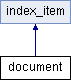
\includegraphics[height=2.000000cm]{classdocument}
\end{center}
\end{figure}
\subsection*{Public Member Functions}
\begin{DoxyCompactItemize}
\item 
\hyperlink{classdocument_af1a85718219b8da6f1befaac0bf87989}{document} ()
\item 
\hyperlink{classdocument_a206a0d6fdb94c618048da73226358ab4}{document} (std\+::string file\+\_\+name)
\item 
virtual unsigned int \hyperlink{classdocument_a45717a4aeff4409b769f0c6f9f72a6f1}{size} () const override
\end{DoxyCompactItemize}
\subsection*{Friends}
\begin{DoxyCompactItemize}
\item 
std\+::ostream \& \hyperlink{classdocument_af474a7f5ba29bca5df031898e86a8687}{operator$<$$<$} (std\+::ostream \&os, const \hyperlink{classdocument}{document} \&doc)
\end{DoxyCompactItemize}
\subsection*{Additional Inherited Members}


\subsection{Constructor \& Destructor Documentation}
\mbox{\Hypertarget{classdocument_af1a85718219b8da6f1befaac0bf87989}\label{classdocument_af1a85718219b8da6f1befaac0bf87989}} 
\index{document@{document}!document@{document}}
\index{document@{document}!document@{document}}
\subsubsection{\texorpdfstring{document()}{document()}\hspace{0.1cm}{\footnotesize\ttfamily [1/2]}}
{\footnotesize\ttfamily document\+::document (\begin{DoxyParamCaption}{ }\end{DoxyParamCaption})}

Default constructor \mbox{\Hypertarget{classdocument_a206a0d6fdb94c618048da73226358ab4}\label{classdocument_a206a0d6fdb94c618048da73226358ab4}} 
\index{document@{document}!document@{document}}
\index{document@{document}!document@{document}}
\subsubsection{\texorpdfstring{document()}{document()}\hspace{0.1cm}{\footnotesize\ttfamily [2/2]}}
{\footnotesize\ttfamily document\+::document (\begin{DoxyParamCaption}\item[{std\+::string}]{file\+\_\+name }\end{DoxyParamCaption})}

constructs a document from a file name 

\subsection{Member Function Documentation}
\mbox{\Hypertarget{classdocument_a45717a4aeff4409b769f0c6f9f72a6f1}\label{classdocument_a45717a4aeff4409b769f0c6f9f72a6f1}} 
\index{document@{document}!size@{size}}
\index{size@{size}!document@{document}}
\subsubsection{\texorpdfstring{size()}{size()}}
{\footnotesize\ttfamily unsigned int document\+::size (\begin{DoxyParamCaption}{ }\end{DoxyParamCaption}) const\hspace{0.3cm}{\ttfamily [override]}, {\ttfamily [virtual]}}

returns the size of the \hyperlink{classindex__item}{index\+\_\+item} 

Implements \hyperlink{classindex__item_ae8ccce55ab973b1a2faa99df65e19051}{index\+\_\+item}.



\subsection{Friends And Related Function Documentation}
\mbox{\Hypertarget{classdocument_af474a7f5ba29bca5df031898e86a8687}\label{classdocument_af474a7f5ba29bca5df031898e86a8687}} 
\index{document@{document}!operator$<$$<$@{operator$<$$<$}}
\index{operator$<$$<$@{operator$<$$<$}!document@{document}}
\subsubsection{\texorpdfstring{operator$<$$<$}{operator<<}}
{\footnotesize\ttfamily std\+::ostream\& operator$<$$<$ (\begin{DoxyParamCaption}\item[{std\+::ostream \&}]{os,  }\item[{const \hyperlink{classdocument}{document} \&}]{doc }\end{DoxyParamCaption})\hspace{0.3cm}{\ttfamily [friend]}}

prints the name of the document with its size 

The documentation for this class was generated from the following files\+:\begin{DoxyCompactItemize}
\item 
project/document.\+hpp\item 
project/document.\+cpp\end{DoxyCompactItemize}

\hypertarget{classindexer}{}\section{indexer Class Reference}
\label{classindexer}\index{indexer@{indexer}}
Inheritance diagram for indexer\+:\begin{figure}[H]
\begin{center}
\leavevmode
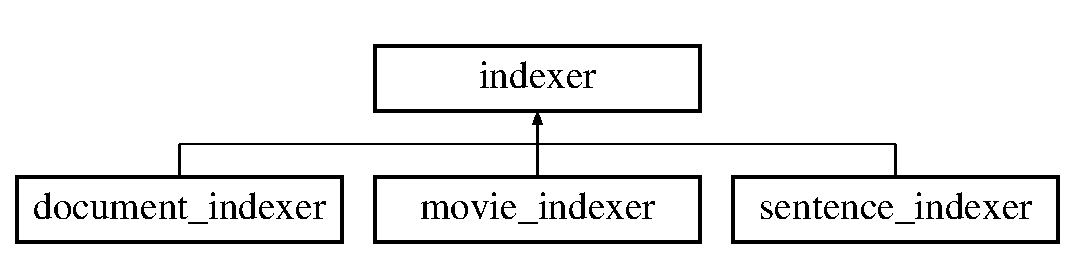
\includegraphics[height=2.000000cm]{classindexer}
\end{center}
\end{figure}
\subsection*{Public Member Functions}
\begin{DoxyCompactItemize}
\item 
\hyperlink{classindexer_acbbcbad080a7ae43ed78840fcf006960}{indexer} ()
\item 
virtual \hyperlink{classindexer_acc872b85bb2520b0cf803801811c9e58}{$\sim$indexer} ()
\item 
void \hyperlink{classindexer_a8c173bf8a59861ffec816f5b79737a6e}{remove\+Stopwords} ()
\item 
const \hyperlink{classindex__item}{index\+\_\+item} $\ast$ \hyperlink{classindexer_a454e14897d75b7a89253e135faaef62a}{operator\mbox{[}$\,$\mbox{]}} (int index) const
\item 
\hyperlink{classindex__item}{index\+\_\+item} $\ast$ \hyperlink{classindexer_abcf129b0575f95fa455b69dfb51edc44}{operator\mbox{[}$\,$\mbox{]}} (int index)
\end{DoxyCompactItemize}
\subsection*{Protected Member Functions}
\begin{DoxyCompactItemize}
\item 
\mbox{\Hypertarget{classindexer_a6e30ca200401d5b7ea2b9fe944d367b6}\label{classindexer_a6e30ca200401d5b7ea2b9fe944d367b6}} 
int {\bfseries size} () const
\item 
\mbox{\Hypertarget{classindexer_a7aa98bdfd37121bbba06127f99325e84}\label{classindexer_a7aa98bdfd37121bbba06127f99325e84}} 
virtual void {\bfseries generate\+Index\+Items} ()=0
\item 
\mbox{\Hypertarget{classindexer_af675f607be274dcd463291963ac3e730}\label{classindexer_af675f607be274dcd463291963ac3e730}} 
virtual std\+::string {\bfseries get\+Index\+File} () const =0
\item 
\mbox{\Hypertarget{classindexer_adc2539219e227f664448927b7337b8dc}\label{classindexer_adc2539219e227f664448927b7337b8dc}} 
virtual std\+::vector$<$ \hyperlink{classquery__result}{query\+\_\+result} $>$ {\bfseries query} (const std\+::string \&q, int n=10)=0
\item 
\mbox{\Hypertarget{classindexer_a31f3dc3a078fb76377a20a56f52e1598}\label{classindexer_a31f3dc3a078fb76377a20a56f52e1598}} 
virtual void {\bfseries generate\+Dictionary} ()
\item 
\mbox{\Hypertarget{classindexer_afd19e249c5224de7b4b308c5420f2412}\label{classindexer_afd19e249c5224de7b4b308c5420f2412}} 
void {\bfseries normalize} ()
\item 
\mbox{\Hypertarget{classindexer_a7cfd3df59433c515df8344196fb2395a}\label{classindexer_a7cfd3df59433c515df8344196fb2395a}} 
double {\bfseries cosine\+\_\+similarity} (const std\+::vector$<$ double $>$ \&q, const std\+::vector$<$ double $>$ \&d, const int doc\+\_\+index)
\end{DoxyCompactItemize}
\subsection*{Protected Attributes}
\begin{DoxyCompactItemize}
\item 
\mbox{\Hypertarget{classindexer_aa48b1798b0488abfedb9d664d2196893}\label{classindexer_aa48b1798b0488abfedb9d664d2196893}} 
dmap {\bfseries dictionary}
\item 
\mbox{\Hypertarget{classindexer_a780732f95bd0822d5b0e7fb81b1569c0}\label{classindexer_a780732f95bd0822d5b0e7fb81b1569c0}} 
std\+::vector$<$ \hyperlink{classindex__item}{index\+\_\+item} $\ast$ $>$ {\bfseries index\+\_\+items}
\item 
\mbox{\Hypertarget{classindexer_ad9beb15bff1c7567dc9869711f82088e}\label{classindexer_ad9beb15bff1c7567dc9869711f82088e}} 
std\+::vector$<$ double $>$ {\bfseries denom\+\_\+double}
\item 
\mbox{\Hypertarget{classindexer_a60d8c3428894603e53b59d5e4146f411}\label{classindexer_a60d8c3428894603e53b59d5e4146f411}} 
std\+::vector$<$ int $>$ {\bfseries totals}
\item 
\mbox{\Hypertarget{classindexer_acecde45d9eddf81e7c241fe8252de998}\label{classindexer_acecde45d9eddf81e7c241fe8252de998}} 
unsigned int {\bfseries max\+Word\+Length}
\item 
\mbox{\Hypertarget{classindexer_a109471f4ff61ac6960845c28bf44cc61}\label{classindexer_a109471f4ff61ac6960845c28bf44cc61}} 
\hyperlink{classstopword}{stopword} {\bfseries stop\+\_\+words}
\end{DoxyCompactItemize}
\subsection*{Friends}
\begin{DoxyCompactItemize}
\item 
\mbox{\Hypertarget{classindexer_a96fe63b3dbcc00194498ff6fc23da381}\label{classindexer_a96fe63b3dbcc00194498ff6fc23da381}} 
std\+::ostream \& {\bfseries operator$<$$<$} (std\+::ostream \&os, const \hyperlink{classindexer}{indexer} \&right)
\item 
\mbox{\Hypertarget{classindexer_a81f04506b77d7cac6b29c6fd84a8665f}\label{classindexer_a81f04506b77d7cac6b29c6fd84a8665f}} 
void {\bfseries operator$>$$>$} (\hyperlink{classindex__item}{index\+\_\+item} \&doc, \hyperlink{classindexer}{indexer} \&idx)
\end{DoxyCompactItemize}


\subsection{Constructor \& Destructor Documentation}
\mbox{\Hypertarget{classindexer_acbbcbad080a7ae43ed78840fcf006960}\label{classindexer_acbbcbad080a7ae43ed78840fcf006960}} 
\index{indexer@{indexer}!indexer@{indexer}}
\index{indexer@{indexer}!indexer@{indexer}}
\subsubsection{\texorpdfstring{indexer()}{indexer()}}
{\footnotesize\ttfamily indexer\+::indexer (\begin{DoxyParamCaption}{ }\end{DoxyParamCaption})}

Default constructor -\/ initializes members \mbox{\Hypertarget{classindexer_acc872b85bb2520b0cf803801811c9e58}\label{classindexer_acc872b85bb2520b0cf803801811c9e58}} 
\index{indexer@{indexer}!````~indexer@{$\sim$indexer}}
\index{````~indexer@{$\sim$indexer}!indexer@{indexer}}
\subsubsection{\texorpdfstring{$\sim$indexer()}{~indexer()}}
{\footnotesize\ttfamily indexer\+::$\sim$indexer (\begin{DoxyParamCaption}{ }\end{DoxyParamCaption})\hspace{0.3cm}{\ttfamily [virtual]}}

Destructor 

\subsection{Member Function Documentation}
\mbox{\Hypertarget{classindexer_a454e14897d75b7a89253e135faaef62a}\label{classindexer_a454e14897d75b7a89253e135faaef62a}} 
\index{indexer@{indexer}!operator\mbox{[}\mbox{]}@{operator[]}}
\index{operator\mbox{[}\mbox{]}@{operator[]}!indexer@{indexer}}
\subsubsection{\texorpdfstring{operator[]()}{operator[]()}\hspace{0.1cm}{\footnotesize\ttfamily [1/2]}}
{\footnotesize\ttfamily const \hyperlink{classindex__item}{index\+\_\+item} $\ast$ indexer\+::operator\mbox{[}$\,$\mbox{]} (\begin{DoxyParamCaption}\item[{int}]{index }\end{DoxyParamCaption}) const}

returns a const pointer to the index item at a given index \mbox{\Hypertarget{classindexer_abcf129b0575f95fa455b69dfb51edc44}\label{classindexer_abcf129b0575f95fa455b69dfb51edc44}} 
\index{indexer@{indexer}!operator\mbox{[}\mbox{]}@{operator[]}}
\index{operator\mbox{[}\mbox{]}@{operator[]}!indexer@{indexer}}
\subsubsection{\texorpdfstring{operator[]()}{operator[]()}\hspace{0.1cm}{\footnotesize\ttfamily [2/2]}}
{\footnotesize\ttfamily \hyperlink{classindex__item}{index\+\_\+item} $\ast$ indexer\+::operator\mbox{[}$\,$\mbox{]} (\begin{DoxyParamCaption}\item[{int}]{index }\end{DoxyParamCaption})}

returns a pointer to the index item at a given index \mbox{\Hypertarget{classindexer_a8c173bf8a59861ffec816f5b79737a6e}\label{classindexer_a8c173bf8a59861ffec816f5b79737a6e}} 
\index{indexer@{indexer}!remove\+Stopwords@{remove\+Stopwords}}
\index{remove\+Stopwords@{remove\+Stopwords}!indexer@{indexer}}
\subsubsection{\texorpdfstring{remove\+Stopwords()}{removeStopwords()}}
{\footnotesize\ttfamily void indexer\+::remove\+Stopwords (\begin{DoxyParamCaption}{ }\end{DoxyParamCaption})}

Removes all stopwords from the dictionary 

The documentation for this class was generated from the following files\+:\begin{DoxyCompactItemize}
\item 
project/indexer.\+hpp\item 
project/indexer.\+cpp\end{DoxyCompactItemize}

\hypertarget{classquery__result}{}\section{query\+\_\+result Class Reference}
\label{classquery__result}\index{query\+\_\+result@{query\+\_\+result}}
\subsection*{Public Member Functions}
\begin{DoxyCompactItemize}
\item 
\mbox{\Hypertarget{classquery__result_a957a24bae5c9fcf83099d7fa2ece2647}\label{classquery__result_a957a24bae5c9fcf83099d7fa2ece2647}} 
{\bfseries query\+\_\+result} (const \hyperlink{classdocument}{document} \&found\+\_\+document, const double score)
\end{DoxyCompactItemize}
\subsection*{Public Attributes}
\begin{DoxyCompactItemize}
\item 
\mbox{\Hypertarget{classquery__result_a2f4b78686ff4f099b298424b9314cee4}\label{classquery__result_a2f4b78686ff4f099b298424b9314cee4}} 
\hyperlink{classdocument}{document} {\bfseries found\+\_\+document}
\item 
\mbox{\Hypertarget{classquery__result_aa385d79066a78d6b47d299ba4bf7f6e4}\label{classquery__result_aa385d79066a78d6b47d299ba4bf7f6e4}} 
double {\bfseries score}
\end{DoxyCompactItemize}
\subsection*{Friends}
\begin{DoxyCompactItemize}
\item 
\mbox{\Hypertarget{classquery__result_af90a86217251694caa9471be14515ee9}\label{classquery__result_af90a86217251694caa9471be14515ee9}} 
bool {\bfseries gt\+Score} (const \hyperlink{classquery__result}{query\+\_\+result} \&left, const \hyperlink{classquery__result}{query\+\_\+result} \&right)
\item 
\mbox{\Hypertarget{classquery__result_aa97ddcf5d38eaf8c7160b9fe609170f5}\label{classquery__result_aa97ddcf5d38eaf8c7160b9fe609170f5}} 
std\+::ostream \& {\bfseries operator$<$$<$} (std\+::ostream \&os, const \hyperlink{classquery__result}{query\+\_\+result} \&qr)
\end{DoxyCompactItemize}


The documentation for this class was generated from the following files\+:\begin{DoxyCompactItemize}
\item 
query\+\_\+result.\+h\item 
query\+\_\+result.\+cpp\end{DoxyCompactItemize}

\hypertarget{classstopword}{}\section{stopword Class Reference}
\label{classstopword}\index{stopword@{stopword}}
\subsection*{Public Member Functions}
\begin{DoxyCompactItemize}
\item 
\mbox{\Hypertarget{classstopword_accb49b6c9d5ddc75002348a869df5619}\label{classstopword_accb49b6c9d5ddc75002348a869df5619}} 
{\bfseries stopword} (const std\+::string \&file\+\_\+name)
\item 
\mbox{\Hypertarget{classstopword_a11210085752c2b3d63055490c13b6666}\label{classstopword_a11210085752c2b3d63055490c13b6666}} 
bool {\bfseries exists} (const std\+::string \&word) const
\item 
\mbox{\Hypertarget{classstopword_a0bee2c17bb62af157dae20b9242805aa}\label{classstopword_a0bee2c17bb62af157dae20b9242805aa}} 
bool {\bfseries operator()} (const std\+::string \&word) const
\end{DoxyCompactItemize}
\subsection*{Friends}
\begin{DoxyCompactItemize}
\item 
\mbox{\Hypertarget{classstopword_a80e1d6c776f6a931100b5ea063e3a6ea}\label{classstopword_a80e1d6c776f6a931100b5ea063e3a6ea}} 
std\+::ostream \& {\bfseries operator$<$$<$} (std\+::ostream \&os, const \hyperlink{classstopword}{stopword} \&sw)
\end{DoxyCompactItemize}


The documentation for this class was generated from the following files\+:\begin{DoxyCompactItemize}
\item 
stopword.\+h\item 
stopword.\+cpp\end{DoxyCompactItemize}

\hypertarget{classtokenizer}{}\section{tokenizer Class Reference}
\label{classtokenizer}\index{tokenizer@{tokenizer}}
\subsection*{Public Member Functions}
\begin{DoxyCompactItemize}
\item 
\hyperlink{classtokenizer_a17c0f75fb81172c979148ae72765c715}{tokenizer} ()
\item 
\hyperlink{classtokenizer_a458162a13637fc34d706f8743ffa8909}{$\sim$tokenizer} ()
\end{DoxyCompactItemize}
\subsection*{Static Public Member Functions}
\begin{DoxyCompactItemize}
\item 
static std\+::vector$<$ std\+::string $>$ \hyperlink{classtokenizer_aa1a768f007e710ff25d63a2cb1de83c3}{tokenize} (const std\+::string \&filename)
\item 
static std\+::string \hyperlink{classtokenizer_a5d553b843e67154be958b849fbf20b62}{sanitize} (std\+::string \&)
\item 
static std\+::vector$<$ std\+::string $>$ \hyperlink{classtokenizer_a9fbc8f511d0eeb0ca2f0333612c99a2a}{tokenize\+\_\+string} (std\+::string \&text)
\end{DoxyCompactItemize}
\subsection*{Friends}
\begin{DoxyCompactItemize}
\item 
std\+::ostream \& \hyperlink{classtokenizer_af8ab6eab63d97d86eb0e8a22eb94aafc}{operator$<$$<$} (std\+::ostream \&os, const \hyperlink{classtokenizer}{tokenizer} \&tk)
\end{DoxyCompactItemize}


\subsection{Constructor \& Destructor Documentation}
\mbox{\Hypertarget{classtokenizer_a17c0f75fb81172c979148ae72765c715}\label{classtokenizer_a17c0f75fb81172c979148ae72765c715}} 
\index{tokenizer@{tokenizer}!tokenizer@{tokenizer}}
\index{tokenizer@{tokenizer}!tokenizer@{tokenizer}}
\subsubsection{\texorpdfstring{tokenizer()}{tokenizer()}}
{\footnotesize\ttfamily tokenizer\+::tokenizer (\begin{DoxyParamCaption}{ }\end{DoxyParamCaption})}

Default constructor \mbox{\Hypertarget{classtokenizer_a458162a13637fc34d706f8743ffa8909}\label{classtokenizer_a458162a13637fc34d706f8743ffa8909}} 
\index{tokenizer@{tokenizer}!````~tokenizer@{$\sim$tokenizer}}
\index{````~tokenizer@{$\sim$tokenizer}!tokenizer@{tokenizer}}
\subsubsection{\texorpdfstring{$\sim$tokenizer()}{~tokenizer()}}
{\footnotesize\ttfamily tokenizer\+::$\sim$tokenizer (\begin{DoxyParamCaption}{ }\end{DoxyParamCaption})}

Destructor 

\subsection{Member Function Documentation}
\mbox{\Hypertarget{classtokenizer_a5d553b843e67154be958b849fbf20b62}\label{classtokenizer_a5d553b843e67154be958b849fbf20b62}} 
\index{tokenizer@{tokenizer}!sanitize@{sanitize}}
\index{sanitize@{sanitize}!tokenizer@{tokenizer}}
\subsubsection{\texorpdfstring{sanitize()}{sanitize()}}
{\footnotesize\ttfamily std\+::string tokenizer\+::sanitize (\begin{DoxyParamCaption}\item[{std\+::string \&}]{text }\end{DoxyParamCaption})\hspace{0.3cm}{\ttfamily [static]}}

removes punctuation and makes all the characters lower case \mbox{\Hypertarget{classtokenizer_aa1a768f007e710ff25d63a2cb1de83c3}\label{classtokenizer_aa1a768f007e710ff25d63a2cb1de83c3}} 
\index{tokenizer@{tokenizer}!tokenize@{tokenize}}
\index{tokenize@{tokenize}!tokenizer@{tokenizer}}
\subsubsection{\texorpdfstring{tokenize()}{tokenize()}}
{\footnotesize\ttfamily std\+::vector$<$ std\+::string $>$ tokenizer\+::tokenize (\begin{DoxyParamCaption}\item[{const std\+::string \&}]{filename }\end{DoxyParamCaption})\hspace{0.3cm}{\ttfamily [static]}}

returns a vector containing all the words (sanitized) from a given file \mbox{\Hypertarget{classtokenizer_a9fbc8f511d0eeb0ca2f0333612c99a2a}\label{classtokenizer_a9fbc8f511d0eeb0ca2f0333612c99a2a}} 
\index{tokenizer@{tokenizer}!tokenize\+\_\+string@{tokenize\+\_\+string}}
\index{tokenize\+\_\+string@{tokenize\+\_\+string}!tokenizer@{tokenizer}}
\subsubsection{\texorpdfstring{tokenize\+\_\+string()}{tokenize\_string()}}
{\footnotesize\ttfamily std\+::vector$<$ std\+::string $>$ tokenizer\+::tokenize\+\_\+string (\begin{DoxyParamCaption}\item[{std\+::string \&}]{text }\end{DoxyParamCaption})\hspace{0.3cm}{\ttfamily [static]}}

returns a vector containing all the words (sanitized) from a given string 

\subsection{Friends And Related Function Documentation}
\mbox{\Hypertarget{classtokenizer_af8ab6eab63d97d86eb0e8a22eb94aafc}\label{classtokenizer_af8ab6eab63d97d86eb0e8a22eb94aafc}} 
\index{tokenizer@{tokenizer}!operator$<$$<$@{operator$<$$<$}}
\index{operator$<$$<$@{operator$<$$<$}!tokenizer@{tokenizer}}
\subsubsection{\texorpdfstring{operator$<$$<$}{operator<<}}
{\footnotesize\ttfamily std\+::ostream\& operator$<$$<$ (\begin{DoxyParamCaption}\item[{std\+::ostream \&}]{os,  }\item[{const \hyperlink{classtokenizer}{tokenizer} \&}]{tk }\end{DoxyParamCaption})\hspace{0.3cm}{\ttfamily [friend]}}

prints the the use of the tokenizer class 

The documentation for this class was generated from the following files\+:\begin{DoxyCompactItemize}
\item 
tokenizer.\+h\item 
tokenizer.\+cpp\end{DoxyCompactItemize}

%--- End generated contents ---

% Index
\backmatter
\newpage
\phantomsection
\clearemptydoublepage
\addcontentsline{toc}{chapter}{Index}
\printindex

\end{document}
